\documentclass[a4paper,12pt]{article}

\usepackage[utf8x]{inputenc}
\usepackage[T2A]{fontenc}
\usepackage[english, russian]{babel}

% Опционно, требует  apt-get install scalable-cyrfonts.*
% и удаления одной строчки в cyrtimes.sty
% Сточку не удалять!
% \usepackage{cyrtimes}

% Картнки и tikz
\usepackage{graphicx}
\usepackage{tikz}
\usetikzlibrary{snakes,arrows,shapes}


% Некоторая русификация.
\usepackage{misccorr}
\usepackage{indentfirst}
\renewcommand{\labelitemi}{\normalfont\bfseries{--}}

% Увы, поля придётся уменьшить из-за листингов.
\topmargin -1cm
\oddsidemargin -0.5cm
\evensidemargin -0.5cm
\textwidth 17cm
\textheight 24cm

\sloppy

% Оглавление в PDF
\usepackage[
bookmarks=true,
colorlinks=true, linkcolor=black, anchorcolor=black, citecolor=black, menucolor=black,filecolor=black, urlcolor=black,
unicode=true
]{hyperref}

% Для исходного кода в тексте
\newcommand{\Code}[1]{\texttt{#1}}


\title{Отчёт по лабораторной работе \\ <<IP-маршрутизация>>}
\author{Фроловский Алексей Вадимович}

\begin{document}

\maketitle

\tableofcontents

\section{Топология сети}

Топология сети и использыемые IP-адреса показаны на рис.~\ref{fig:network}.

\begin{figure}
\centering
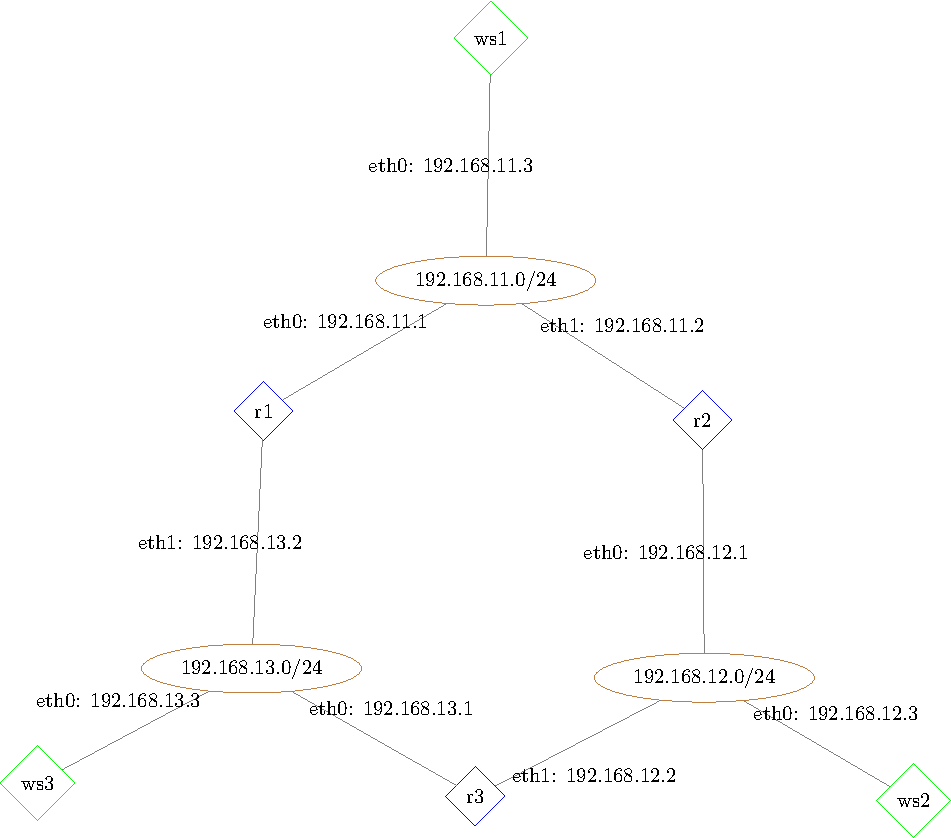
\includegraphics[width=\textwidth]{includes/network_gv.pdf}
\caption{Топология сети}
\label{fig:network}
\end{figure}


\section{Назначение IP-адресов}

Ниже приведён файл настройки протокола IP маршрутизатора \textbf{r1}:

\begin{Verbatim}
auto lo
iface lo inet loopback

auto eth0
iface eth0 inet static
address 192.168.11.1
netmask 255.255.255.0
up ip r add 192.168.12.0/24 via 192.168.11.2 dev eth0
down ip r del 192.168.12.0/24

auto eth1
iface eth1 inet static
address 192.168.13.2
netmask 255.255.255.0
\end{Verbatim}

Ниже приведён файл настройки протокола IP маршрутизатора \textbf{r2}:

\begin{Verbatim}
auto lo
iface lo inet loopback

auto eth0
iface eth0 inet static
address 192.168.12.1
netmask 255.255.255.0
up ip r add 192.168.13.0/24 via 192.168.12.2 dev eth0
down ip r del 192.168.13.0/24

auto eth1
iface eth1 inet static
address 192.168.11.2
netmask 255.255.255.0
\end{Verbatim}

Ниже приведён файл настройки протокола IP маршрутизатора \textbf{r3}:

\begin{Verbatim}
auto lo
iface lo inet loopback

auto eth0
iface eth0 inet static
address 192.168.13.1
netmask 255.255.255.0
up ip r add 192.168.11.0/24 via 192.168.13.2 dev eth0
down ip r del 192.168.11.0/24

auto eth1
iface eth1 inet static
address 192.168.12.2
netmask 255.255.255.0
\end{Verbatim}

Ниже приведён файл настройки протокола IP рабочей станции \textbf{ws1}:

\begin{Verbatim}
auto lo
iface lo inet loopback

auto eth0
iface eth0 inet static
address 192.168.11.3
netmask 255.255.255.0
up ip r add 192.168.12.0/24 via 192.168.11.2 dev eth0
down ip r del 192.168.12.0/24
gateway 192.168.11.1
\end{Verbatim}

Ниже приведён файл настройки протокола IP рабочей станции \textbf{ws2}:

\begin{Verbatim}
auto lo
iface lo inet loopback

auto eth0
iface eth0 inet static
address 192.168.12.3
netmask 255.255.255.0
up ip r add 192.168.13.0/24 via 192.168.12.2 dev eth0
down ip r del 192.168.13.0/24
gateway 192.168.12.1
\end{Verbatim}

Ниже приведён файл настройки протокола IP рабочей станции \textbf{ws3}:

\begin{Verbatim}
auto lo
iface lo inet loopback

auto eth0
iface eth0 inet static
address 192.168.13.3
netmask 255.255.255.0
up ip r add 192.168.11.0/24 via 192.168.13.2 dev eth0
down ip r del 192.168.11.0/24
gateway 192.168.13.1
\end{Verbatim}

\section{Таблица маршрутизации}

Ниже показана таблица маршрутизации для маршрутизатора \textbf{r1}:

\begin{Verbatim}
192.168.13.0/24 dev eth1  proto kernel  scope link  src 192.168.13.2 
192.168.12.0/24 via 192.168.11.2 dev eth0 
192.168.11.0/24 dev eth0  proto kernel  scope link  src 192.168.11.1
\end{Verbatim}

Ниже показана таблица маршрутизации для маршрутизатора \textbf{r2}:

\begin{Verbatim}
192.168.13.0/24 via 192.168.12.2 dev eth0 
192.168.12.0/24 dev eth0  proto kernel  scope link  src 192.168.12.1 
192.168.11.0/24 dev eth1  proto kernel  scope link  src 192.168.11.2
\end{Verbatim}

Ниже показана таблица маршрутизации для маршрутизатора \textbf{r3}:

\begin{Verbatim}
192.168.13.0/24 dev eth0  proto kernel  scope link  src 192.168.13.1 
192.168.12.0/24 dev eth1  proto kernel  scope link  src 192.168.12.2 
192.168.11.0/24 via 192.168.13.2 dev eth0
\end{Verbatim}

Ниже показана таблица маршрутизации для рабочей станции \textbf{ws1}:

\begin{Verbatim}
192.168.12.0/24 via 192.168.11.2 dev eth0 
192.168.11.0/24 dev eth0  proto kernel  scope link  src 192.168.11.3 
default via 192.168.11.1 dev eth0
\end{Verbatim}

Ниже показана таблица маршрутизации для рабочей станции \textbf{ws2}:

\begin{Verbatim}
192.168.13.0/24 via 192.168.12.2 dev eth0 
192.168.12.0/24 dev eth0  proto kernel  scope link  src 192.168.12.3 
default via 192.168.12.1 dev eth0
\end{Verbatim}

Ниже показана таблица маршрутизации для рабочей станции \textbf{ws3}:

\begin{Verbatim}
192.168.13.0/24 dev eth0  proto kernel  scope link  src 192.168.13.3 
192.168.11.0/24 via 192.168.13.2 dev eth0 
default via 192.168.13.1 dev eth0
\end{Verbatim}

\section{Проверка настройки сети}

Вывод \textbf{traceroute} от узла \textbf{ws1} до узла \textbf{ws2} при нормальной работе сети:

\begin{Verbatim}
traceroute to 192.168.12.3 (192.168.12.3), 64 hops max, 40 byte packets
 1  192.168.11.2  6 ms  1 ms  1 ms
 2  192.168.12.3  13 ms  1 ms  1 ms
\end{Verbatim}

Вывод \textbf{traceroute} от маршрутизатора \textbf{r1} до узла \textbf{ws2} при нормальной работе сети:

\begin{Verbatim}
traceroute to 192.168.12.3 (192.168.12.3), 64 hops max, 40 byte packets
 1  192.168.11.2  7 ms  0 ms  0 ms
 2  192.168.12.3  11 ms  1 ms  0 ms
\end{Verbatim}

Вывод \textbf{traceroute} от узла \textbf{ws1} до узла \textbf{ws3} при нормальной работе сети:

\begin{Verbatim}
traceroute to 192.168.13.3 (192.168.13.3), 64 hops max, 40 byte packets
 1  192.168.11.1  6 ms  1 ms  1 ms
 2  192.168.13.3  12 ms  1 ms  1 ms
\end{Verbatim}

Вывод \textbf{traceroute} от узла \textbf{ws2} до узла \textbf{ws1} при нормальной работе сети:

\begin{Verbatim}
traceroute to 192.168.11.3 (192.168.11.3), 64 hops max, 40 byte packets
 1  192.168.12.1  1 ms  1 ms  1 ms
 2  192.168.11.3  2 ms  2 ms  1 ms
\end{Verbatim}

Вывод \textbf{traceroute} от узла \textbf{ws2} до узла \textbf{ws3} при нормальной работе сети:

\begin{Verbatim}
traceroute to 192.168.13.3 (192.168.13.3), 64 hops max, 40 byte packets
 1  192.168.12.2  13 ms  1 ms  1 ms
 2  192.168.13.3  13 ms  1 ms  1 ms
\end{Verbatim}

Вывод \textbf{traceroute} от маршрутизатора \textbf{r2} до узла \textbf{ws3} при нормальной работе сети:

\begin{Verbatim}
traceroute to 192.168.13.3 (192.168.13.3), 64 hops max, 40 byte packets
 1  192.168.12.2  3 ms  0 ms  0 ms
 2  192.168.13.3  11 ms  0 ms  0 ms
\end{Verbatim}

Вывод \textbf{traceroute} от узла \textbf{ws3} до узла \textbf{ws1} при нормальной работе сети:

\begin{Verbatim}
traceroute to 192.168.11.3 (192.168.11.3), 64 hops max, 40 byte packets
 1  192.168.13.2  1 ms  1 ms  1 ms
 2  192.168.11.3  2 ms  2 ms  1 ms
\end{Verbatim}

Вывод \textbf{traceroute} от маршрутизатора \textbf{r3} до узла \textbf{ws1} при нормальной работе сети:

\begin{Verbatim}
traceroute to 192.168.11.3 (192.168.11.3), 64 hops max, 40 byte packets
 1  192.168.13.2  1 ms  1 ms  0 ms
 2  192.168.11.3  1 ms  1 ms  1 ms
\end{Verbatim}

Вывод \textbf{traceroute} от узла \textbf{ws3} до узла \textbf{ws2} при нормальной работе сети:

\begin{Verbatim}
traceroute to 192.168.12.3 (192.168.12.3), 64 hops max, 40 byte packets
 1  192.168.13.1  1 ms  1 ms  1 ms
 2  192.168.12.3  2 ms  1 ms  2 ms
\end{Verbatim}

\section{Маршрутизация}

Маршрутизатор \textbf{r1} имеет следующие параметры сетевых интерфейсов:

\begin{Verbatim}
1: lo: <LOOPBACK,UP,LOWER_UP> mtu 16436 qdisc noqueue 
    link/loopback 00:00:00:00:00:00 brd 00:00:00:00:00:00
    inet 127.0.0.1/8 scope host lo
    inet6 ::1/128 scope host 
       valid_lft forever preferred_lft forever
2: teql0: <NOARP> mtu 1500 qdisc noop qlen 100
    link/void 
3: eth0: <BROADCAST,MULTICAST,UP,LOWER_UP> mtu 1500 qdisc pfifo_fast qlen 1000
    link/ether 0e:ab:f8:0c:10:4b brd ff:ff:ff:ff:ff:ff
    inet 192.168.11.1/24 brd 192.168.11.255 scope global eth0
    inet6 fe80::cab:f8ff:fe0c:104b/64 scope link 
       valid_lft forever preferred_lft forever
4: eth1: <BROADCAST,MULTICAST,UP,LOWER_UP> mtu 1500 qdisc pfifo_fast qlen 1000
    link/ether fa:de:dc:30:96:57 brd ff:ff:ff:ff:ff:ff
    inet 192.168.13.2/24 brd 192.168.13.255 scope global eth1
    inet6 fe80::f8de:dcff:fe30:9657/64 scope link 
       valid_lft forever preferred_lft forever
\end{Verbatim}

Таблица маршрутизации для \textbf{r1} имеет следующий вид:

\begin{Verbatim}
192.168.13.0/24 dev eth1  proto kernel  scope link  src 192.168.13.2 
192.168.12.0/24 via 192.168.11.2 dev eth0 
192.168.11.0/24 dev eth0  proto kernel  scope link  src 192.168.11.1
\end{Verbatim}

Маршрутизатор \textbf{r2} имеет следующие параметры сетевых интерфейсов:

\begin{Verbatim}
1: lo: <LOOPBACK,UP,LOWER_UP> mtu 16436 qdisc noqueue 
    link/loopback 00:00:00:00:00:00 brd 00:00:00:00:00:00
    inet 127.0.0.1/8 scope host lo
    inet6 ::1/128 scope host 
       valid_lft forever preferred_lft forever
2: teql0: <NOARP> mtu 1500 qdisc noop qlen 100
    link/void 
3: eth0: <BROADCAST,MULTICAST,UP,LOWER_UP> mtu 1500 qdisc pfifo_fast qlen 1000
    link/ether 3a:40:ee:31:9e:cd brd ff:ff:ff:ff:ff:ff
    inet 192.168.12.1/24 brd 192.168.12.255 scope global eth0
    inet6 fe80::3840:eeff:fe31:9ecd/64 scope link 
       valid_lft forever preferred_lft forever
4: eth1: <BROADCAST,MULTICAST,UP,LOWER_UP> mtu 1500 qdisc pfifo_fast qlen 1000
    link/ether 12:3e:e2:7d:e3:87 brd ff:ff:ff:ff:ff:ff
    inet 192.168.11.2/24 brd 192.168.11.255 scope global eth1
    inet6 fe80::103e:e2ff:fe7d:e387/64 scope link 
       valid_lft forever preferred_lft forever
\end{Verbatim}

Таблица маршрутизации для \textbf{r2} имеет следующий вид:

\begin{Verbatim}
192.168.13.0/24 via 192.168.12.2 dev eth0 
192.168.12.0/24 dev eth0  proto kernel  scope link  src 192.168.12.1 
192.168.11.0/24 dev eth1  proto kernel  scope link  src 192.168.11.2
\end{Verbatim}

Рабочая станция \textbf{ws1} имеет следующие параметры сетевых интерфейсов:

\begin{Verbatim}
1: lo: <LOOPBACK,UP,LOWER_UP> mtu 16436 qdisc noqueue 
    link/loopback 00:00:00:00:00:00 brd 00:00:00:00:00:00
    inet 127.0.0.1/8 scope host lo
    inet6 ::1/128 scope host 
       valid_lft forever preferred_lft forever
2: teql0: <NOARP> mtu 1500 qdisc noop qlen 100
    link/void 
3: eth0: <BROADCAST,MULTICAST,UP,LOWER_UP> mtu 1500 qdisc pfifo_fast qlen 1000
    link/ether a6:f9:52:b6:1e:69 brd ff:ff:ff:ff:ff:ff
    inet 192.168.11.3/24 brd 192.168.11.255 scope global eth0
    inet6 fe80::a4f9:52ff:feb6:1e69/64 scope link 
       valid_lft forever preferred_lft forever
\end{Verbatim}

Таблица маршрутизации для \textbf{ws1} имеет следующий вид:

\begin{Verbatim}
192.168.12.0/24 via 192.168.11.2 dev eth0 
192.168.11.0/24 dev eth0  proto kernel  scope link  src 192.168.11.3 
default via 192.168.11.1 dev eth0
\end{Verbatim}

Рабочая станция \textbf{ws2} имеет следующие параметры сетевых интерфейсов:

\begin{Verbatim}
1: lo: <LOOPBACK,UP,LOWER_UP> mtu 16436 qdisc noqueue 
    link/loopback 00:00:00:00:00:00 brd 00:00:00:00:00:00
    inet 127.0.0.1/8 scope host lo
    inet6 ::1/128 scope host 
       valid_lft forever preferred_lft forever
2: teql0: <NOARP> mtu 1500 qdisc noop qlen 100
    link/void 
3: eth0: <BROADCAST,MULTICAST,UP,LOWER_UP> mtu 1500 qdisc pfifo_fast qlen 1000
    link/ether da:53:12:09:ea:4e brd ff:ff:ff:ff:ff:ff
    inet 192.168.12.3/24 brd 192.168.12.255 scope global eth0
    inet6 fe80::d853:12ff:fe09:ea4e/64 scope link 
       valid_lft forever preferred_lft forever
\end{Verbatim}

Далее показана отправка пакета с рабочей станции \textbf{ws1} на рабочую станцию
\textbf{ws2} (после стирания кеша ARP) для демонстрации косвенной маршрутизации:

\begin{Verbatim}
ping 192.168.12.3 -c 1
\end{Verbatim}

На первом шаге рабочая станция \textbf{ws1} определяет по своей маршрутной таблице,
что пакет нужно отправить на адрес 192.168.11.2. Затем рабочая станция \textbf{ws1} 
пытается узнать MAC-адрес с помощью протокола ARP и отправляет сам пакет на
маршрутизатор \textbf{r2}:

\begin{Verbatim}
a6:f9:52:b6:1e:69 > ff:ff:ff:ff:ff:ff, ethertype ARP (0x0806), length 42:
    arp who-has 192.168.11.2 tell 192.168.11.3
12:3e:e2:7d:e3:87 > a6:f9:52:b6:1e:69, ethertype ARP (0x0806), length 42:
    arp reply 192.168.11.2 is-at 12:3e:e2:7d:e3:87
a6:f9:52:b6:1e:69 > 12:3e:e2:7d:e3:87, ethertype IPv4 (0x0800), length 98:
    192.168.11.3 > 192.168.12.3: ICMP echo request, id 24322, seq 1, length 64
\end{Verbatim}

После чего маршрутизатор \textbf{r2}, находящийся в одном сегменте сети с рабочей
станцией \textbf{ws2}, определяет MAC-адрес получателя и отправляет непосредственно
сам пакет получателю:

\begin{Verbatim}
3a:40:ee:31:9e:cd > ff:ff:ff:ff:ff:ff, ethertype ARP (0x0806), length 42: 
    arp who-has 192.168.12.3 tell 192.168.12.1
da:53:12:09:ea:4e > 3a:40:ee:31:9e:cd, ethertype ARP (0x0806), length 42:
    arp reply 192.168.12.3 is-at da:53:12:09:ea:4e
3a:40:ee:31:9e:cd > da:53:12:09:ea:4e, ethertype IPv4 (0x0800), length 98:
    192.168.11.3 > 192.168.12.3: ICMP echo request, id 24322, seq 1, length 64
\end{Verbatim}

\section{Продолжительность жизни пакета}

Создадим маршрутную петлю между маршрутизаторами \textbf{r1} и \textbf{r2}. Для этого
отключим на маршрутизаторе \textbf{r2} интерфейс eth0 и добавим неверный маршрут 
до сети 192.168.12.0:

\begin{Verbatim}
ip link set eth0 down
ip route add 192.168.12.0/24 via 192.168.11.1 dev eth1
\end{Verbatim}

После чего таблица маршрутизации для маршрутизатора \textbf{r2} будет иметь следующий вид:

\begin{Verbatim}
192.168.12.0/24 via 192.168.11.1 dev eth1 
192.168.11.0/24 dev eth1  proto kernel  scope link  src 192.168.11.2
\end{Verbatim}

С рабочей станции \textbf{ws1} пошлeм эхо-запрос на рабочую станцию \textbf{ws2}:

\begin{Verbatim}
ping 192.168.12.3 -c 1
\end{Verbatim}

Ниже приведены перемещения пакета с эхо-запросом по маршрутной петле, из которых
видно, что сообщение об истечении жизни пакета было отправлено с маршрутизатора
\textbf{r1}:

\begin{Verbatim}
a6:f9:52:b6:1e:69 > 12:3e:e2:7d:e3:87, ethertype IPv4 (0x0800), length 98:
    (tos 0x0, ttl 64, id 0, offset 0, flags [DF], proto ICMP (1), length 84) 
    192.168.11.3 > 192.168.12.3: ICMP echo request, id 8450, seq 1, length 64
12:3e:e2:7d:e3:87 > 0e:ab:f8:0c:10:4b, ethertype IPv4 (0x0800), length 98:
    (tos 0x0, ttl 63, id 0, offset 0, flags [DF], proto ICMP (1), length 84)
    192.168.11.3 > 192.168.12.3: ICMP echo request, id 8450, seq 1, length 64
\vdots
0e:ab:f8:0c:10:4b > 12:3e:e2:7d:e3:87, ethertype IPv4 (0x0800), length 98:
    (tos 0x0, ttl 2, id 0, offset 0, flags [DF], proto ICMP (1), length 84)
    192.168.11.3 > 192.168.12.3: ICMP echo request, id 8450, seq 1, length 64
12:3e:e2:7d:e3:87 > 0e:ab:f8:0c:10:4b, ethertype IPv4 (0x0800), length 98:
    (tos 0x0, ttl 1, id 0, offset 0, flags [DF], proto ICMP (1), length 84)
    192.168.11.3 > 192.168.12.3: ICMP echo request, id 8450, seq 1, length 64
0e:ab:f8:0c:10:4b > a6:f9:52:b6:1e:69, ethertype IPv4 (0x0800), length 126:
    (tos 0xc0, ttl 64, id 15633, offset 0, flags [none], proto ICMP (1), length 112)
    192.168.11.1 > 192.168.11.3: ICMP time exceeded in-transit, length 92
	    (tos 0x0, ttl 1, id 0, offset 0, flags [DF], proto ICMP (1), length 84)
	    192.168.11.3 > 192.168.12.3: ICMP echo request, id 8450, seq 1, length 64
\end{Verbatim}

\section{Изучение IP-фрагментации}

Для изучения фрагментации IP-пакетов выполним следующие действия:

\begin{itemize}

\item Изменим маршрут следования пакетов между узлами \textbf{ws1} и \textbf{ws2} сети 
       таким образом, чтобы пакеты, между этими сетями проходили через маршртизаторы 
       \textbf{r1} и \textbf{r3}. Для этого выполним следуюшие дествия:

\begin{itemize}

\item Удалим маршрут следования пакетов из сети 192.168.11.0/24 в сеть
       192.168.12.0/24 через маршрутизатор \textbf{r2} из маршрутной таблицы
       рабочей станции \textbf{ws1} и маршрутизатора \textbf{r1}:

\begin{Verbatim}
ip route del 192.168.12.0/24 via 192.168.11.2 dev eth0
\end{Verbatim}

\item Добавим маршрут следования пакетов из сети 192.168.11.0/24 в сеть
       192.168.12.0/24 через маршрутизатор \textbf{r3} в маршрутную таблицу
       маршрутизатора \textbf{r1}:

\begin{Verbatim}
ip route add 192.168.12.0/24 via 192.168.13.1 dev eth1
\end{Verbatim}

\end{itemize}

\item Уменьшим величину MTU в сети между маршрутизаторами \textbf{r1} и \textbf{r3}. 
       Поскольку все подключенные к одному сегменту сетевые интерфейсы должны иметь 
       одинаковое представление о величине MTU сегмента, то выполним следующие действия:
       
\begin{itemize}

\item Уменьшим величину MTU на интерфейсе eth1 маршрутизатора \textbf{r1}:

\begin{Verbatim}
ip link set dev eth1 mtu 576
\end{Verbatim}

\item Уменьшим величину MTU на интерфейсе eth0 маршрутизатора \textbf{r3} и рабочей 
         станции \textbf{ws3}:

\begin{Verbatim}
ip link set dev eth0 mtu 576
\end{Verbatim}

\end{itemize}

\item Отключим механизм борьбы с фрагменацией на рабочей станции \textbf{ws1}:

\begin{Verbatim}
echo 1 > /proc/sys/net/ipv4/ip_no_pmtu_disc
\end{Verbatim}

\end{itemize}

Для тестиования отправим эхо-запрос с рабочей станции \textbf{ws1} на рабочую станцию
\textbf{ws2}:

\begin{Verbatim}
ping -c 1 -s 1000 192.168.12.3
\end{Verbatim}

Вывод \textbf{tcpdump} на маршрутизаторе \textbf{r1} (перед сетью с уменьшенным MTU):

\begin{Verbatim}
IP (tos 0x0, ttl 64, id 16587, offset 0, flags [none], proto ICMP (1), length 1028)
    192.168.11.3 > 192.168.12.3: ICMP echo request, id 11266, seq 1, length 1008
\end{Verbatim}

Вывод \textbf{tcpdump} на маршрутизаторе \textbf{r3} (после сети с уменьшенным MTU):

\begin{Verbatim}
IP (tos 0x0, ttl 63, id 16587, offset 0, flags [+], proto ICMP (1), length 572)
    192.168.11.3 > 192.168.12.3: ICMP echo request, id 11266, seq 1, length 552
IP (tos 0x0, ttl 63, id 16587, offset 552, flags [none], proto ICMP (1), length 476)
    192.168.11.3 > 192.168.12.3: icmp
\end{Verbatim}

Вывод \textbf{tcpdump} на узле получателя:

\begin{Verbatim}
IP (tos 0x0, ttl 62, id 16587, offset 0, flags [none], proto ICMP (1), length 1028)
    192.168.11.3 > 192.168.12.3: ICMP echo request, id 11266, seq 1, length 1008
\end{Verbatim}

\section{Отсутствие сети}

Для проведения опыта отключим на маршрутизаторе \textbf{r2} интерфейс eth0:

\begin{Verbatim}
ip link set eth0 down
\end{Verbatim}

Затем отправим пакет с эхо-запросом с рабочей станции \textbf{ws1} на рабочую станцию
\textbf{ws2}:

\begin{Verbatim}
ping 192.168.12.3 -c 1
\end{Verbatim}

Вывод \textbf{ping} на рабочей станции \textbf{ws1}:

\begin{Verbatim}
PING 192.168.12.3 (192.168.12.3) 56(84) bytes of data.
From 192.168.11.2 icmp_seq=1 Destination Net Unreachable

--- 192.168.12.3 ping statistics ---
1 packets transmitted, 0 received, +1 errors, 100\% packet loss, time 0ms
\end{Verbatim}

Вывод \textbf{tcpdump} на маршрутизаторе \textbf{r2}:

\begin{Verbatim}
IP (tos 0x0, ttl 64, id 0, offset 0, flags [DF], proto ICMP (1), length 84)
    192.168.11.3 > 192.168.12.3: ICMP echo request, id 5378, seq 1, length 64
IP (tos 0xc0, ttl 64, id 60546, offset 0, flags [none], proto ICMP (1), length 112)
    192.168.11.2 > 192.168.11.3: ICMP net 192.168.12.3 unreachable, length 92
	    IP (tos 0x0, ttl 64, id 0, offset 0, flags [DF], proto ICMP (1), length 84)
	        192.168.11.3 > 192.168.12.3: ICMP echo request, id 5378, seq 1, length 64
\end{Verbatim}

\section{Отсутствие IP-адреса в сети}

Для проведения опыта отправим пакет с эхо-запросом с рабочей станции \textbf{ws1} в сеть
192.168.12.0/24 на несущесвующий узел 192.168.12.4:

\begin{Verbatim}
ping 192.168.12.4 -c 1
\end{Verbatim}

Вывод \textbf{ping} на рабочей станции \textbf{ws1}:

\begin{Verbatim}
PING 192.168.12.4 (192.168.12.4) 56(84) bytes of data.
From 192.168.11.2 icmp_seq=1 Destination Host Unreachable

--- 192.168.12.4 ping statistics ---
1 packets transmitted, 0 received, +1 errors, 100\% packet loss, time 0ms
\end{Verbatim}

Вывод \textbf{tcpdump} на маршрутизаторе \textbf{r2}:

\begin{Verbatim}
IP (tos 0x0, ttl 64, id 0, offset 0, flags [DF], proto ICMP (1), length 84)
    192.168.11.3 > 192.168.12.4: ICMP echo request, id 5634, seq 1, length 64
IP (tos 0xc0, ttl 64, id 36124, offset 0, flags [none], proto ICMP (1), length 112)
    192.168.11.2 > 192.168.11.3: ICMP host 192.168.12.4 unreachable, length 92
	    IP (tos 0x0, ttl 63, id 0, offset 0, flags [DF], proto ICMP (1), length 84)
	        192.168.11.3 > 192.168.12.4: ICMP echo request, id 5634, seq 1, length 64
\end{Verbatim}

\end{document}
